% !TEX root = ../dg.tex

\section{Homogeneous Manifolds}
\label{sec:homogeneous manifolds}

Given a group $G$ and a normal subgroup $N$, it's a standard fact from algebra that the quotient (i.e., collection of cosets) $G/N$ is also a group. The key point is that, for $g_1, g_2 \in G$, the coset $(g_1 N) (g_2 N) := g_1 g_2 N$ is well-defined: for $n_1,n_2 \in N$, we can write $n_1 = g_2 n g_2^{-1}$ for  $n := g_2^{-1} n_1 g_2 \in N$, so
\[
	(g_1 n_1) (g_2 n_2) = (g_1 g_2 n g_2^{-1}) (g_2 n_2) = (g_1 g_2) (n n_2) \in g_1 g_2 N.
\]

The same holds true for Lie groups: if $G$ is a Lie group and $N$ is a normal Lie subgroup, then $G/N$ is a Lie group. For example, $\SL_n(\R)$ is a closed normal subgroup of $\GL_n(\R)$, and 
\[
	\GL_n(\R) / \SL_n(\R) \cong \R^\times = \GL_1(\R),
\]
the multiplicative group of nonzero real numbers

Okay, but what if we take a Lie subgroup $H$ of a Lie group $G$ which is not normal? Does the coset space $G/H$ have any special structure? Not surprisingly, given how I've set it up, the answer is yes:

\begin{theorem}\label{thm:homogeneous space}
	Let $H$ be a closed subgroup of a Lie group $G$ (i.e., a Lie subgroup) and let $G/H$ be the set of left cosets $\{gH : g \in G\}$. If $\pi \from G \to G/H$ is the obvious map, then $G/H$ has a unique manifold structure so that
	\begin{enumerate}
		\item $\pi$ is smooth and
		\item there exist local sections of $G/H$: for $gH \in G/H$, there exists a neighborhood $U$ of $gH$ and a smooth map $\sigma \from U \to G$ so that $\pi \circ \sigma = \operatorname{id}|_U$.
	\end{enumerate}
\end{theorem}

The proof of this theorem is kind of a pain, so we skip it. Manifolds of the form $G/H$ are called \emph{homogeneous manifolds} (or sometimes \emph{homogeneous spaces}).

\begin{example}\label{ex:S^2 as homogeneous space}
	Let $G = \SO(3)$ and let $H = \left\{\begin{bmatrix} \cos \theta & -\sin \theta & 0 \\ \sin \theta & \cos \theta & 0 \\ 9 & 0 & 1 \end{bmatrix} : \theta \in \R \right\}$. Then the theorem says that $G/H$ is a manifold. 
	
	Which one? Well, think about the usual action of $\SO(3)$ on $\R^3$ (or equivalently, by \Cref{ex:adjoint action of so3}, the adjoint representation of $\SO(3)$). If we pick $v = (0,0,1) \in R^3$, then the orbit $G \cdot v = \{ g \cdot v : g \in \SO(3)\}$ (i.e., the adjoint orbit of the corresponding element of $\mathfrak{so}(3)$) will consist of all vectors with the same norm as $v$; in other words, it is the standard sphere of radius 1. Moreover, the action of $H$ on $v$ is trivial: $H \cdot v = \{v\}$. So it is not insane to guess that the elements of $G/H$ are in one-to-one correspondence with the points on the sphere.
	
	Indeed, this is true: define the map $\phi \from \SO(3)/H \to S^2$ by
	\[
		gH \mapsto g \cdot v.
	\]
	I claim this is a diffeomorphism, so there are a bunch of things to check:
	\begin{description}
		\item[$\phi$ is well-defined:] For $h \in H$, $\phi(ghH) = (gh) \cdot v = g \cdot (h \cdot v) = g \cdot v = \phi(gH)$ since $h \cdot v = v$.
		\item[$\phi$ is surjective:] It's geometrically clear that the action of $\SO(3)$ on $S^2$ is transitive, but let's actually see this explicitly. Suppose $u \in S^2$. If $u = (0,0,\pm 1)$ and $g = \begin{bmatrix} \pm 1 & 0 & 0 \\ 0 & 1 & 0 \\ 0 & 0 & \pm 1 \end{bmatrix}$, then $g \cdot v = u$. Otherwise, $u = (x,y,z)$ where $x^2 + y^2 > 0$. If $\theta$ is the angle between $u$ and $v$, then $\cos \theta = u \cdot v = z$ and $x^2 + y^2 = 1-z^2 = 1-\cos^2\theta = \sin^2\theta$. Define $n := \frac{u \times v}{\|u \times v\|} = \frac{(y,-x,0)}{\sqrt{x^2 + y^2}}$, and let $N$ be the corresponding element of $\mathfrak{so}(3)$:
		\[
			N = \begin{bmatrix} 0 & 0 & \frac{-x}{\sqrt{x^2+y^2}} \\
			0 & 0 & \frac{-y}{\sqrt{x^2+y^2}} \\
			\frac{x}{\sqrt{x^2+y^2}} & \frac{y}{\sqrt{x^2+y^2}} & 0 \end{bmatrix}.
		\]
		% Likewise, let
		% \[
		% 	U = \begin{bmatrix} 0 & -z & y \\
		% 	z & 0 & -x \\
		% 	-y & x & 0 \end{bmatrix}
		% \]
		% be the element of $\mathfrak{so}(3)$ corresponding to $u$.
		Then I claim that $e^{-\theta N}v = u$. To see this, we can use \Cref{ex:general one-parameter subgroup of SO(3)} to compute 
		\begin{multline*}
			e^{-\theta N}v  = \cos (-\theta)v + \sin (-\theta) n \times v + (1-\cos (-\theta)) (v \cdot n) n  \\
			= (\cos \theta)\begin{bmatrix} 0  \\ 0 \\ 1 \end{bmatrix} - \frac{ \sin \theta}{\sqrt{x^2 + y^2}}\begin{bmatrix} -x \\ -y \\ \cos \theta -z \end{bmatrix} + 0  = \begin{bmatrix} x \\ y \\ z \end{bmatrix}  = u
		\end{multline*}
		since $n \times v = (u \times v) \times v = (u \cdot v) v - (v \cdot v) u = (\cos \theta)v - u$ and $\sqrt{x^2+y^2} = \sin\theta$.
		
		\item[$\phi$ is injective:] Suppose $\phi(g_1 H) = \phi(g_2 H)$. Then
		\[
			\phi(g_2^{-1} g_1 H) = (g_2^{-1} g_1) \cdot v = g_2^{-1} \cdot (g_1 \cdot v) = g_2^{-1} \cdot \phi(g_1 H) = g_2^{-1} \cdot \phi(g_2 H) = g_2^{-1} \cdot (g_2 \cdot v) = (g_2^{-1} g_2) \cdot v = v
		\]
		so $g_2^{-1} g_1 \in H$ (since $H$ consists of all elements of $\SO(3)$ fixing $v$), and hence $g_2 H = g_2g_2^{-1} g_1 H = g_1 H$.
		\item[$\phi$ is smooth:] If $\pi \from \SO(3) \to \SO(3)/H$ is the projection, then I claim that $\phi$ is smooth if and only if $\phi \circ \pi$ is smooth.
		\ifplastex
		\begin{figure}[htbp]
			\centering
				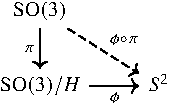
\includegraphics[height=1in]{proj-cd}
			\caption{$\phi$, $\pi$, and the map to $S^2$.}
			\alttext{A commutative diagram with $\SO(3)$ is the upper-left, $\SO(3)/H$ is the lower-left, and $S^2$ in the lower-right. There is an arrow labeled $\pi$ from $\SO(3)$ to $\SO(3)/H$, and arrow labeled $\phi$ from $\SO(3)/H$ to $S^2$, and a dashed arrow labeled $\phi \circ \pi$ from $\SO(3)$ to $S^2$.}
			\label{fig:proj-cd}
		\end{figure}
		\else	
			\[
				\begin{tikzcd}
					\SO(3)  \arrow[d,"\pi"'] \arrow[dr,"\phi \circ \pi",dashed] \\
					\SO(3)/H \arrow[r,"\phi"'] & S^2 
				\end{tikzcd}
			\]
		\fi
		If $\phi$ is smooth then $\phi \circ \pi$ is clearly smooth since $\pi$ is. On the other hand, if $\phi \circ \pi$ is smooth, then on a neighborhood $U$ of $gH \in \SO(3)/H$ with local section $\sigma \from U \to \SO(3)$ we have that
		\[
			(\phi \circ \pi) \circ \sigma = \phi \circ (\pi \circ \sigma) = \phi \circ \operatorname{id}|_U = \phi|_U
		\]
		is smooth. Since such local sections exist at all points (by \Cref{thm:homogeneous space}), $\phi$ is smooth. But now it's clear that $(\phi \circ \pi)(g) = g \cdot v$ is smooth since the rotation action on $S^2$ is smooth, and therefore $\phi$ is smooth.
		
		\item[$\phi$ has smooth inverse:] We know $\phi$ is bijective, so it has an inverse, and the only challenge is to show that the inverse is smooth. By the inverse function theorem, it suffices to show that $d\phi$ is nonsingular everywhere, or equivalently that $\ker d(\phi \circ \pi)_g \subset T_g H \subset T_g \SO(3)$. Now, for $g \in \SO(3)$,
		\begin{multline*}
			(\phi \circ \pi)(g) = \phi(\pi(g)) = \phi(gH) = g \cdot v = g \cdot (I \cdot v) = g \cdot (\phi(H)) = g \cdot((\phi \circ \pi)(I)) \\
			= g \cdot\left((\phi \circ \pi)\left(g^{-1} g\right)\right) = g \cdot \left(\left(\phi \circ \pi \circ L_{g^{-1}}\right)(g)\right),
		\end{multline*}
		so it suffices to show this at the identity: $\ker d(\phi \circ \pi)_I \subset T_I H$. So now let $U = \begin{bmatrix} 0 & -z & y \\ z & 0 & -x \\ -y & x & 0 \end{bmatrix} \in T_I \SO(3)$, corresponding to the vector $u = (x,y,z) \in S^2$. We know that $U = \alpha'(0)$ where $\alpha(t) = e^{tU}$, so
		\begin{multline*}
			d(\phi \circ \pi)_I (U) = ((\phi \circ \pi) \circ \alpha)'(0) = \left. \frac{d}{dt} \right|_{t=0} \phi(\pi(\alpha(t))) \\
			= \left. \frac{d}{dt}\right|_{t=0} \phi(\pi(e^{tU})) = \left. \frac{d}{dt}\right|_{t=0} \phi(e^{tU}H) = \left. \frac{d}{dt}\right|_{t=0} e^{tU}\cdot v.
		\end{multline*}
		Again, we can use \Cref{ex:general one-parameter subgroup of SO(3)} to compute
		\[
			e^{tU}\cdot v = (\cos t) v + (\sin t) u \times v + (1-\cos t)(v \cdot u)u = \begin{bmatrix} y \sin t + xz(1-\cos t) \\ -x \sin t + yz(1-\cos t) \\ z \cos t + z^2(1-\cos t) \end{bmatrix},
		\]
		so
		\[
			d(\phi \circ \pi)_I (U) = \left. \frac{d}{dt}\right|_{t=0} \begin{bmatrix} y \sin t + xz(1-\cos t) \\ -x \sin t + yz(1-\cos t) \\ z \cos t + z^2(1-\cos t) \end{bmatrix} = \begin{bmatrix} y \\ -x \\ 0 \end{bmatrix}.
		\]
		So $U \in \ker d(\phi \circ \pi)_I$ if and only if $x=y=0$, meaning that $U = \begin{bmatrix} 0 & -z & 0 \\ z & 0 & 0 \\ 0 & 0 & 0 \end{bmatrix}$, which is indeed in the tangent space to $H$. 
		
		Thus, we can conclude that $d\phi$ is nonsingular everywhere and hence the inverse is smooth.
	\end{description}
\end{example}

Essentially the same argument gives a much more general result, which we need one definition in order to state:

\begin{definition}\label{def:isotropy subgroup}
	If $M$ is a manifold and $G$ is a Lie group which acts smoothly on $M$, the \emph{isotropy subgroup} of $G$ at a point $p \in M$ is the group
	\[
		G_p = \{g\in G : g \cdot p = p\}.
	\]
\end{definition}

(Incidentally, this induces the \emph{isotropy representation} $G_p \to \Aut(T_pM)$ given by $g \mapsto \left.(d \phi_g)_p \right|_{T_pM}$, where $\phi_g(q) := g \cdot q$ for all $q \in M$.)

\begin{theorem}\label{thm:homogeneous and isotropy}
	Suppose a Lie group $G$ acts transitively on a manifold $M$ and that, for some $p \in M$, $H = G_p$ is the isotropy subgroup for $p$. Then $M$ is diffeomorphic to $G/H$.
\end{theorem}

Indeed, most books define \emph{homogeneous manifolds} to be manifolds admitting a smooth, transitive action of a Lie group, which explains the name: since the group action is transitive, every point is in some sense the same as every other point. \Cref{thm:homogeneous and isotropy} tells us that our definition of homogeneous manifold and the standard definition are equivalent.

\begin{example}
	The same reasoning as in \Cref{ex:S^2 as homogeneous space} shows that $S^n \cong \SO(n+1)/\SO(n)$.
\end{example}

\begin{example}
	Consider $\U(n+1)$ acting on the unit sphere $S^{2n+1} \subset \C^{n+1}$. The isotropy subgroup of the north pole is the subgroup
	\[
		\left\{ \begin{bmatrix} U & 0 \\ 0 & 1 \end{bmatrix} : U \in \U(n)\right\},
	\]
	so $S^{2n+1} \cong \U(n+1)/\U(n)$.
	
	Consider the special case when $n=0$. Then this says $S^1 \cong \U(1)/\U(0)$, which is obviously true since $\U(0) = \{1\}$ and $\U(1)$ is just the unit complex numbers; i.e., the unit circle.
\end{example}

\begin{example}
	Similarly, $S^{2n+1} \cong \SU(n+1)/\SU(n)$. In the special case $n=1$, we get 
	\[
		S^3 \cong \SU(2)/\SU(1) = \SU(2)/\{1\} \cong \SU(2),
	\]
	which gives a simple proof of a fact we've alluded to many times.
\end{example}